%%%%%%%%%%%%%%%%%%%%%%%%%%%%%%%%% COMMENT THIS TO COMPILE main.tex %%%%%%%%%%%%%%%%%%%%%%%%%%%%%%%%
%\documentclass[a4paper,12pt]{report}
\usepackage[english]{babel}
\usepackage[left=2cm,right=2cm,top=2cm,bottom=2cm]{geometry}
%\usepackage{mathtools}
\usepackage{amsthm}     % for definitions and theorems
\usepackage[many]{tcolorbox}    % boxes around definitions and theorems
%\usepackage{amsmath}
%\usepackage{nccmath}
\usepackage{amssymb}    % \ltimes
\usepackage{etoolbox}   % for start of Chapter
%\usepackage{amsfonts}
\usepackage{physics}    % for all Physics related
\usepackage{dsfont}     % for the identity matrix symbol \1
%\usepackage{mathrsfs}

\usepackage{titling}
\usepackage{indentfirst}

\usepackage{bm}
\usepackage[dvipsnames]{xcolor}
\usepackage{cancel}

\usepackage{xurl}
\usepackage[colorlinks=true]{hyperref}

\usepackage{float}
\usepackage{graphicx}
\usepackage{subcaption}
%\usepackage{tikz}

\usepackage{ctable}     % tabelas
\renewcommand{\P}{\phantom{+}}  % empty space to indent things
\usepackage{multirow}
\usepackage{tabulary}

%%%%%%%%%%%%%%%%%%%%%%%%%%%%%%%%%%%%%%%%%%%%%%%%%%%

\newcommand{\eps}{\epsilon}
\newcommand{\vphi}{\varphi}
\newcommand{\cte}{\text{cte}}

\newcommand{\N}{{\mathbb{N}}}
\newcommand{\Z}{{\mathbb{Z}}}
%\newcommand{\Q}{{\mathbb{Q}}}
\newcommand{\C}{{\mathbb{C}}}
\renewcommand{\S}{{\hat{S}}}
%\renewcommand{\H}{\s{H}}

\renewcommand{\a}{{\vb{a}}}
\renewcommand{\b}{{\vb{b}}}
\renewcommand{\d}{{\dagger}}
\newcommand{\up}{{\uparrow}}
\newcommand{\down}{{\downarrow}}
\newcommand{\hc}{{\text{h.c.}}}

\newcommand{\ihat}{\bm{\hat{\imath}}}
\newcommand{\jhat}{\bm{\hat{\jmath}}}
\newcommand{\khat}{\bm{\hat{k}}}

\newcommand{\0}{{\vb{0}}}
\newcommand{\1}{\mathds{1}}
\newcommand{\E}{{\vb{E}}}
\newcommand{\B}{{\vb{B}}}
\renewcommand{\u}{{\vb{u}}}
\renewcommand{\v}{{\vb{v}}}
\renewcommand{\r}{{\vb{r}}}
\newcommand{\R}{{\vb{R}}}
\newcommand{\Q}{{\vb{Q}}}
\newcommand{\G}{{\vb{G}}}
\newcommand{\g}{{\vb{g}}}
\renewcommand{\k}{{\vb{k}}}
\newcommand{\K}{{\vb{K}}}
\newcommand{\p}{{\vb{p}}}
\newcommand{\q}{{\vb{q}}}
\newcommand{\F}{{\vb{F}}}
\renewcommand{\t}{{\vb{t}}}
\newcommand{\vtau}{{\bm{\tau}}}
\newcommand{\vdelta}{{\bm{\delta}}}

% COLORED SYMMETRY ELEMENTS
\newcommand{\Ct}{{\textcolor{Cyan}{C_3}}}
\newcommand{\Ctn}[1]{{\textcolor{Cyan}{C_3^{\textcolor{black}{#1}}}}}
\newcommand{\Cs}{{\textcolor{ForestGreen}{C_6}}}
\newcommand{\Csn}[1]{{\textcolor{ForestGreen}{C_6^{\textcolor{black}{#1}}}}}
\newcommand{\sd}{{\textcolor{RoyalBlue}{\sigma_d}}}
\newcommand{\sdn}[1]{{\textcolor{RoyalBlue}{\sigma_d^{\textcolor{black}{#1}}}}}
\newcommand{\sdp}{{\textcolor{RoyalBlue}{\sigma_d'}}}
\newcommand{\sdpp}{{\textcolor{RoyalBlue}{\sigma_d''}}}
\newcommand{\sv}{{\textcolor{Orange}{\sigma_v}}}
\newcommand{\svn}[1]{{\textcolor{Orange}{\sigma_v^{\textcolor{black}{#1}}}}}
\newcommand{\svp}{{\textcolor{Orange}{\sigma_v'}}}
\newcommand{\svpp}{{\textcolor{Orange}{\sigma_v''}}}

\newcommand{\s}{\sigma}
%\newcommand{\prodint}[2]{\left\langle #1 , #2 \right\rangle}
\newcommand{\cc}[1]{\overline{#1}}
\newcommand{\Eval}[3]{\eval{\left( #1 \right)}_{#2}^{#3}}
\newcommand{\sg}[2]{\{ #1 \mid #2 \}}

\newcommand{\unit}[1]{\; \mathrm{#1}}

\newcommand{\n}{\medskip}
\newcommand{\e}{\quad \mathrm{and} \quad}
\newcommand{\ou}{\quad \mathrm{or} \quad}
\newcommand{\virg}{\, , \;}
\newcommand{\ptodo}{\forall \,}
\renewcommand{\implies}{\; \Rightarrow \;}
%\newcommand{\eqname}[1]{\tag*{#1}} % Tag equation with name

\setlength{\droptitle}{-7em}

\makeatletter
\patchcmd{\chapter}{\if@openright\cleardoublepage\else\clearpage\fi}{}{}{}  % start 'Chapter' at the same page. needs package etoolbox
\makeatother

%% Theorems, definitions, proofs
\theoremstyle{definition}

\newtheorem{definition}{Definition}[section]
\tcolorboxenvironment{definition}{
  colback=blue!5!white,
  boxrule=0pt,
  boxsep=1pt,
  left=2pt,right=2pt,top=2pt,bottom=2pt,
  oversize=2pt,
  sharp corners,
  before skip=\topsep,
  after skip=\topsep,
}

\newtheorem{theorem}{Theorem}[section]
\tcolorboxenvironment{theorem}{
  colback=blue!5!white,
  boxrule=0pt,
  boxsep=1pt,
  left=2pt,right=2pt,top=2pt,bottom=2pt,
  oversize=2pt,
  sharp corners,
  before skip=\topsep,
  after skip=\topsep,
}

%\begin{document}
%%%%%%%%%%%%%%%%%%%%%%%%%%%%%%%%% COMMENT THIS TO COMPILE main.tex %%%%%%%%%%%%%%%%%%%%%%%%%%%%%%%%


%%%%%%%%%%%%%%%%%%%%%%%%%%%%%%%%%%%%%%%%%%%%%%%%%%%%%%%%%%%%%%%%%%%%%%%%%%%%%%%%%%%%%%%%%%%%%%%%%%
\chapter{Introduction}
%%%%%%%%%%%%%%%%%%%%%%%%%%%%%%%%%%%%%%%%%%%%%%%%%%%%%%%%%%%%%%%%%%%%%%%%%%%%%%%%%%%%%%%%%%%%%%%%%%

Carbon is undoubtedly one of the most essential elements for the formation of life, largely due to its remarkable versatility in bonding, which enables the formation of a vast array of complex compounds. Among materials composed solely of carbon atoms, graphite is one of which we are very familiar since elementary school, as it used in pencils for drawing. Graphite is an allotrope of carbon, consisting of multiple layers stacked together and held by weak van der Waals forces. When writing with a pencil, some graphite layers transfer onto the paper, allowing for drawing and writing.

In 2004, Andre Geim, Konstantin Novoselov, et. al. \cite{novoselov_2004} successfully isolated a single sheet of graphite using the ``sticky tape method'', allowing them to study its properties. This single atomic layer, known as graphene, was the first two-dimensional (2D) material ever discovered. Graphene exhibits extraordinary properties, including exceptional electrical conductivity, mechanical strength, flexibility, transparency, and thermal conductivity. Its unique combination of properties makes it a promising candidate for a wide range of applications, from electronics and energy storage to composite materials and biomedical devices. The discovery of graphene marked a breakthrough, inaugurating the field of 2D materials and earning Geim and Novoselov the Nobel Prize in Physics in 2010.

When we vertically stack a few layers of 2D materials, the system is held together by weak van der Waals forces and is known as a van der Waals heterostructure. These heterostructures represent a promising new avenue for engineering the properties of 2D materials. While the properties of single-layer materials, such as graphene, are now well understood, predicting the behavior of few-layer heterostructures remains challenging. <++>

%%%%%%%%%%%%%%%%%%%%%%%%%%%%%%%%%%%%%%%%%%%%%%%%%%%%%%%%%%%%%%%%%%%%%%%%%%%%%%%%%%%%%%%%%%%%%%%%%%
\section{Monolayer}
%%%%%%%%%%%%%%%%%%%%%%%%%%%%%%%%%%%%%%%%%%%%%%%%%%%%%%%%%%%%%%%%%%%%%%%%%%%%%%%%%%%%%%%%%%%%%%%%%%

Throughout our work, $\hbar = 1$.

\n

Graphene is an allotrope of graphite and consists of a hexagonal lattice of carbon atoms linked in $sp^2$ hybridization with distance $a$, where $3$ electrons from carbon form $\s$ bonds and the last electron is located on a $\pi$ orbital and is the only one that matters for the electronic properties of the material.

\n

Our convention is zig-zag in horizontal direction and arm-chair in vertical direction.

\begin{figure}[H]
\centering
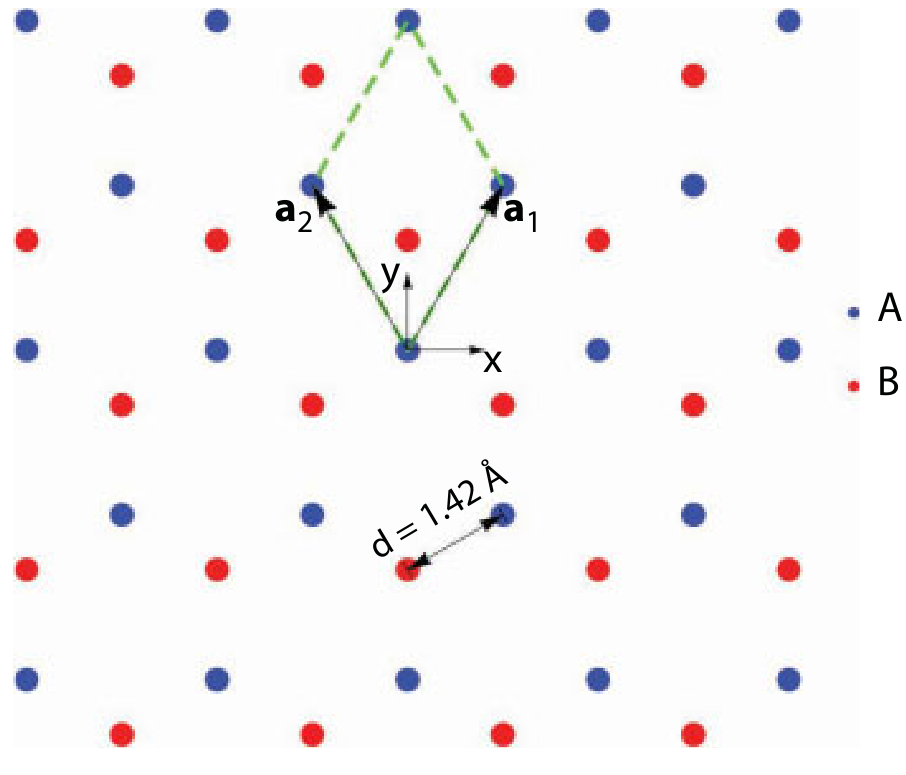
\includegraphics[width=0.4\linewidth]{fig/graphene-lattice_vectors2.png}
\label{fig:graphene-lattice_vectors}
\caption{\textcolor{red}{Graphene lattice vectors. Taken from \cite{handbook2019}}}
\end{figure}

The lattice vectors are $\vb{a}_1 = a \qty(\frac{1}{2}, \frac{\sqrt{3}}{2})$, $\vb{a}_2 = a \qty(-\frac{1}{2}, \frac{\sqrt{3}}{2})$. The unit cell area is $ A_1 = \abs{\a_1 \times \a_2} = \frac{\sqrt{3}}{2} a^2 $.

The Brillouin zone is
\begin{figure}[H]
\centering
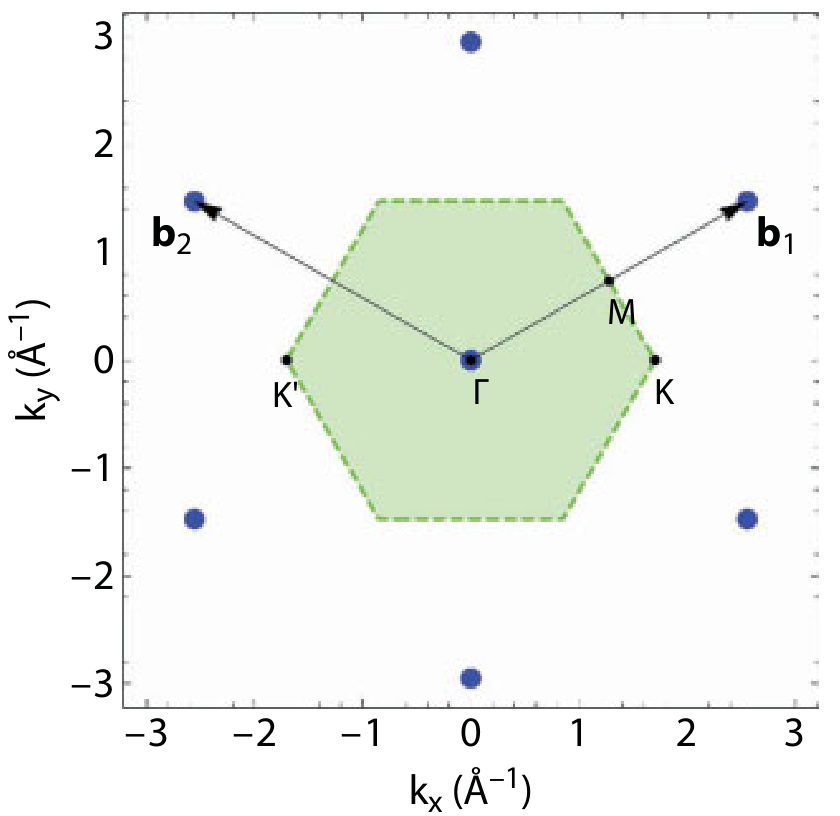
\includegraphics[width=0.3\linewidth]{fig/brillouin-zone-monolayer.png}
\caption{\textcolor{red}{Graphene Brillouin Zone. Taken from \cite{handbook2019}}}
\label{fig:brillouin-zone-monolayer}
\end{figure}

Using the convention $\a_3 = \vu{z}$, the momentum lattice vectors are
\begin{equation} \label{eq:monolayer-bvecs}
\b_1 = \frac{2\pi}{A_1} \a_2 \times \a_3 = \frac{4\pi}{\sqrt{3} a } \qty(\frac{\sqrt{3}}{2}, \frac{1}{2}), \quad
\b_2 = \frac{2\pi}{A_1} \a_3 \times \a_1 = \frac{4\pi}{\sqrt{3} a } \qty(-\frac{\sqrt{3}}{2}, \frac{1}{2}).
\end{equation}

The two main Dirac points are defined as
\begin{equation} \label{eq:monolayer-dirac-points}
\K = \frac{4\pi}{3a} (1, 0) , \quad \K' = -\K.
\end{equation}



We write a tight-binding hamiltonian with only nearest-neighbor hopping
\begin{equation} \label{eq:monolayer-tight-binding}
H = -t \sum_{\R} c^\d_B(\R) \qty(c_A(\R) + c_A(\R-\a_1) + c_A(\R-\a_2)) + \hc,
\end{equation}
where the $\R$ sum runs through all the associated Bravais triangular lattice. Applying the Fourier transforms
\begin{equation} \label{eq:monolayer-fourier}
c_{\alpha}^\d(\R) = \frac{1}{\sqrt{N}} \sum_{\k \in \text{BZ}} e^{-i \k \vdot \r_i} c_A^\d(\k),
\end{equation}
we get
\begin{equation} \label{eq:monolayer-tight-binding2}
H = \sum_{\k}
\begin{pmatrix}
c_A^\d(\k) & c_B^\d(\k)
\end{pmatrix}
\begin{pmatrix}
0 & -t f(\k) \\
-t f^*(\k) & 0
\end{pmatrix}
\begin{pmatrix}
c_A^\d(\k) \\ c_B^\d(\k)
\end{pmatrix},
\end{equation}
with
\begin{equation} \label{eq:monolayer-fk}
f(\k) = \sum_{\nu} e^{i \k \vdot \bm{\delta}_\nu} =
e^{idk_y} + 2 e^{-\frac{idk_y}{2}} \cos(\frac{\sqrt{3}}{2} dk_x),
\end{equation}
where $\bm{\delta}_1 = (\a_1 + \a_2)/3 = d (0, 1)$, $\bm{\delta}_2 = (-2\a_1 + \a_2)/3 = d(-\frac{\sqrt{3}}{2}, -\frac{1}{2})$, $\bm{\delta}_3 = (\a_1 - 2\a_2)/3 = d (\frac{\sqrt{3}}{2}, -\frac{1}{2})$ are the vectors that connect to the three nearest neighboring sites, and $d = a/\sqrt{3}$.

\n

The eigenenergies of hamiltonian \ref{eq:monolayer-tight-binding2} are $E_\pm(\k) = \pm t \abs{f(\k)}$. Notice that the points $\K$ and $\K'=-\K$ are roots of $f$, i.e., $f(\pm\K) = 0$. These are the so-called Dirac points, around which the dispersion relation are approximately linear $E(\K + \q) = v_F \abs{\q} + O(\abs{\q}/\abs{\K})^2$.

%%%%%%%%%%%%%%%%%%%%%%%%%%%%%%%%%%%%%%%%%%%%%%%%%%%%%%%%%%%%%%%%%%%%%%%%%%%%%%%%%%%%%%%%%%%%%%%%%%%
%\section{AB stacking}
%%%%%%%%%%%%%%%%%%%%%%%%%%%%%%%%%%%%%%%%%%%%%%%%%%%%%%%%%%%%%%%%%%%%%%%%%%%%%%%%%%%%%%%%%%%%%%%%%%%
%
%The so-called Bernal or AB stacking of two layers of graphene is such that the atoms of sublattice $A$ from one layer are placed above the atoms of sublattice $B$ from the other layer.
%To model the bilayer system in this configuration, we use the monolayer tight-binding hamiltonian (with only the first
%nearest neighbors) as a basis and include an interlayer hopping. Indexing the layers with $\ell = 1, 2$, we write
%\begin{equation} \label{eq:ab-hamil}
%H = H_1 + H_2 + H_{\perp},
%\end{equation}
%\begin{equation} \label{eq:ab-slg-hamil}
%\begin{split}
%H_\ell &= -t \sum_{\R} c_{\ell,A}^\d(\R) [c_{\ell,B}(\R) + c_{\ell,B}(\R-\a_1) + c_{\ell,B}(\R-\a_2)] + \hc, \\
%H_\perp &= t_{\perp} \sum_{\R} c_{1,A}^\d(\R) c_{2,B}(\R) + \hc,
%\end{split}
%%\begin{split}
%%H_1 &= -t \sum_{\R} c_{1,A}^\d(\R) [c_{1,B}(\R) + c_{1,B}(\R-\a_1) + c_{1,B}(\R-\a_2)] + \hc, \\
%%H_2 &= -t \sum_{\R} c_{2,A}^\d(\R) [c_{2,B}(\R) + c_{2,B}(\R-\a_1) + c_{2,B}(\R-\a_2)] + \hc,
%%\end{split}
%\end{equation}
%where $c_{\ell,\alpha}(\R)^\d$ is the creation operator for an electron in a state $\ket{\ell,\R,\alpha}$. Using the discrete Fourier Transform of the creation operators
%\begin{equation} \label{eq:ft-creatio}
%c_{\ell,\alpha}^\d(\R) = \frac{1}{\sqrt{N}} \sum_{\k\in\text{1BZ}} e^{-i\k\vdot(\R+\bm{\tau}_{\ell,\alpha})} c_{\ell,\alpha}^\d(\k),
%\end{equation}
%we can rewrite $H = \sum_{\k} \Psi^\d(\k) H(\k) \Psi(\k)$, where $\Psi^\d(\k) = (c_{1,A}^\d(\k) \; c_{1,B}^\d(\k) \; c_{2,A}^\d(\k) \; c_{2,B}^\d(\k))$ and
%\begin{equation} \label{eq:ab-momentum_space}
%H(\k) =
%\begin{pmatrix}
%0 & -t f(\k) & 0 & t_\perp \\
%-t f^*(\k) & 0 & 0 & 0 \\
%0 & 0 & 0 & -t f(\k) \\
%t_\perp & 0 & -t f^*(\k) & 0 \\
%\end{pmatrix}.
%\end{equation}
%
%Diagonalizing $H(\k)$ we obtain the four bands for the AB-stacked bilayer graphene
%\begin{equation} \label{eq:ab-four_bands}
%E_{\pm,\pm} = \pm t
%\sqrt{
%\qty(\frac{t_\perp}{2t})^2 +
%4 \cos(\frac{\sqrt{3}}{2} d \, k_x) \cos(\frac{3}{2} d \, k_y) + 2 \cos(\sqrt{3} d \, k_x) + 3
%}
%\; \pm \; \frac{t_\perp}{2}.
%\end{equation}

%%%%%%%%%%%%%%%%%%%%%%%%%%%%%%%%%%%%%%%%%%%%%%%%%%%%%%%%%%%%%%%%%%%%%%%%%%%%%%%%%%%%%%%%%%%%%%%%%%
\section{Commensurate Angles}
%%%%%%%%%%%%%%%%%%%%%%%%%%%%%%%%%%%%%%%%%%%%%%%%%%%%%%%%%%%%%%%%%%%%%%%%%%%%%%%%%%%%%%%%%%%%%%%%%%

\begin{figure}[H]
\centering
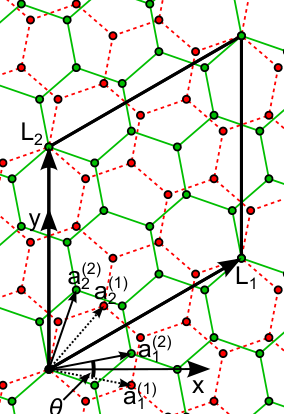
\includegraphics[width=0.4\textwidth]{fig/latvec.png}
\caption{Commensurate angle case and lattice vectors. Taken from \cite{koshino2012}}
\label{fig:latvec}
\end{figure}

As drawn in Figure \ref{fig:latvec}, we have
\begin{align}
\label{eq:scalarprods0}
\abs{\a_i^{(j)}} &= a, \\
\label{eq:scalarprods1}
\vb{a}_1^{(j)} \vdot \vb{a}_2^{(j)} &= a^2 \cos(60^\circ) = a^2/2, \\
\label{eq:scalarprods2}
\vb{a}_1^{(1)} \vdot \vb{a}_1^{(2)} &= a^2 \cos\theta, \\
\label{eq:scalarprods3}
\vb{a}_1^{(1)} \vdot \vb{a}_2^{(2)} &= a^2 \cos(60^\circ + \theta), \\
\label{eq:scalarprods4}
\vb{a}_1^{(2)} \vdot \vb{a}_2^{(1)} &= a^2 \cos(60^\circ - \theta).
\end{align}

The superlattice vectors $\vb{L}_1$, $\vb{L}_2$ (when the angle is commensurate) are related by a $60^\circ$ rotation. In general, because $\vb{L}_1$ is a point that belongs to the lattices of both layers, it is written by integers $m,n,m',n'$ as
\begin{equation} \label{eq:L1}
\vb{L}_1 = m\vb{a}_1^{(1)} + n\vb{a}_2^{(1)} = m'\vb{a}_1^{(2)} + n'\vb{a}_2^{(2)}.
\end{equation}

Koshino \cite{koshino2012} argues that there is an appropriate choice of lattice vectors $\vb{a}_1^{(1)}, \vb{a}_2^{(1)}, \vb{a}_1^{(2)}, \vb{a}_2^{(2)}$ (satisfying equations \ref{eq:scalarprods0} to \ref{eq:scalarprods4}) such that the indices $(m',n')$ can be made equal to $(n,m)$. By taking the scalar products of equation \ref{eq:L1} with $\vb{a}_1^{(1)}$ and $\vb{a}_1^{(2)}$, we get
$$
\begin{cases}
\; m + n/2 = n \cos\theta + m \cos(60^\circ + \theta); \\
\; m/2 + n = m \cos\theta + n \cos(60^\circ - \theta).
\end{cases}
\Rightarrow
\begin{cases}
\; mn + n^2/2 = n^2 \cos\theta + mn \qty(\frac{\cos\theta}{2}
- \frac{\sqrt{3} \sin\theta}{2}); \\
\; m^2/2 + mn = m^2 \cos\theta + mn \qty(\frac{\cos\theta}{2}
+ \frac{\sqrt{3} \sin\theta}{2}).
\end{cases}
$$

Summing the two equations above gives us
\begin{equation} \label{eq:costheta}
\boxed{\cos\theta = \frac{1}{2} \cdot \frac{m^2 + n^2 + 4mn}{m^2 + n^2 + mn}.}
\end{equation}

If $d = \gcd(m, n) > 1$, we can take new integers $M = m/d$, $N = n/d$, and $\vb{L}_1' = M\vb{a}_1^{(1)} + N\vb{a}_2^{(1)} = N\vb{a}_1^{(2)} + M\vb{a}_2^{(2)}$, such that $\gcd(M, N) = 1$. Therefore, the shortest translation vector of equation \ref{eq:L1} is obtained by coprime integers $m, n$. Now, substituting $n = m + r$ we get
\begin{equation} \label{eq:costheta-r}
\boxed{\cos\theta = \frac{1}{2} \cdot \frac{m^2 + (m^2 + 2mr + r^2) + 4m^2 + 4mr}{m^2 + (m^2 + 2mr + r^2) + m^2 + mr} =
\frac{3 m^2 + 3mr + r^2/2}{3m^2 + 3mr + r^2}. }
\end{equation}

Because $\gcd(m, n) = \gcd(m, n-m) = \gcd(m, r)$, we also get that $m$ and $r$ are coprime integers.

\n

\boxed{\textbf{CHECAR SE HÁ DIFERENÇA NA DEDUÇÃO PARA TIPO I E TIPO II.}}


%%%%%%%%%%%%%%%%%%%%%%%%%%%%%%%%%%%%%%%%%%%%%%%%%%%%%%%%%%%%%%%%%%%%%%%%%%%%%%%%%%%%%%%%%%%%%%%%%%
\section{Moiré pattern}
%%%%%%%%%%%%%%%%%%%%%%%%%%%%%%%%%%%%%%%%%%%%%%%%%%%%%%%%%%%%%%%%%%%%%%%%%%%%%%%%%%%%%%%%%%%%%%%%%%

By taking the norm of $\vb{L}_1$ from equation \ref{eq:L1} and using the angle relation in equation \ref{eq:costheta}, we find that the superlattice constant $L = \abs{\vb{L}_1} = \abs{\vb{L}_2}$ is given by
$$
2\sin[2](\theta/2) = 1 - \cos\theta = \frac{(m-n)^2}{2(m^2+n^2+mn)} \implies
\sqrt{m^2+n^2+mn} = \frac{\abs{m-n}}{2\sin(\theta/2)} \implies
$$
\begin{equation} \label{eq:L-commensurate}
L = a\sqrt{m^2 + n^2 + mn} = \frac{\abs{m-n}}{2 \sin(\theta/2)} \, a.
\end{equation}

\n


The area of an unit cell of the superlattice is $A = \frac{\sqrt{3}}{2} L^2 = (m^2 + n^2 + mn) \, A_1$, where $A_1 = \frac{\sqrt{3}}{2} \, a^2$ is the area of unit cell of monolayer graphene. If we consider now the area of the Brillouin Zone, we get
\begin{equation} \label{eq:bz-volume}
\Omega = \frac{\Omega_1}{m^2 + n^2 + mn},
\end{equation}
where $\Omega_1 = (2\pi)^2/A$ is the BZ area of the monolayer and $\Omega$ is the area of the moiré mini BZ.

\n

For example, $(m,n) = (1,2)$ and $\theta = 21.8^\circ$ we have $m^2 + n^2 + mn = 7$, therefore the monolayer BZ fits 7 mini BZ's in its area, as we see in Figure \ref{fig:bzminibz}.
\begin{figure}[H]
\centering
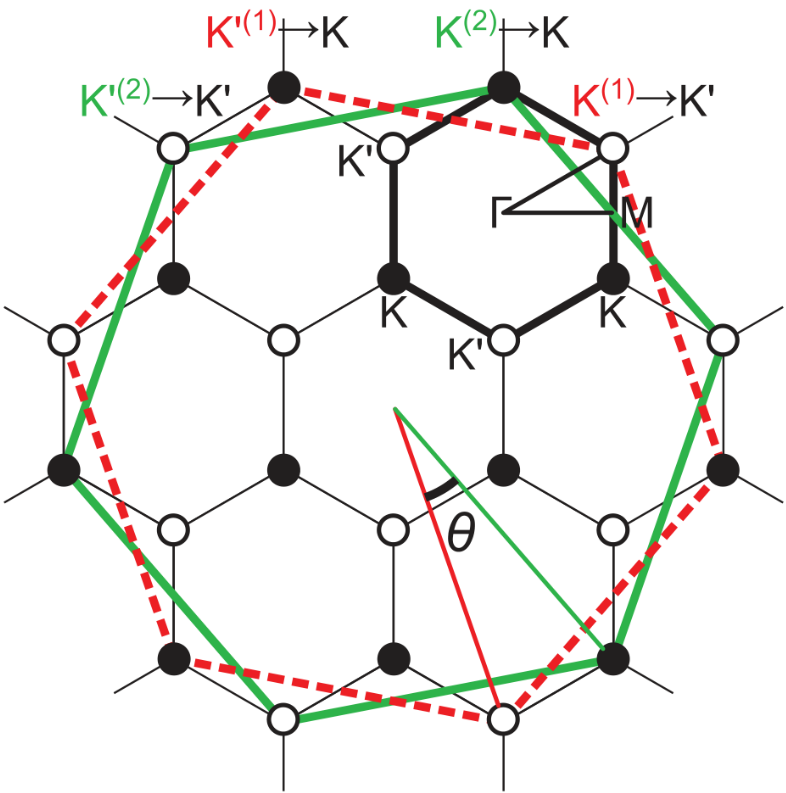
\includegraphics[width=0.5\linewidth]{fig/bzminibz.png}
\caption{Monolayers (red and green) and mini BZ's with $(m,n) = (1,2)$ and $\theta = 21.8^\circ$. Taken from \cite{koshino2012}.}
\label{fig:bzminibz}
\end{figure}

\n

\textbf{WHY DO WE ONLY CONSIDERER $\abs{m-n} = 1$?} Type I and Type II angles from Zou.

%%%%%%%%%%%%%%%%%%%%%%%%%%%%%%%%%%%%%%%%%%%%%%%%%%%%%%%%%%%%%%%%%%%%%%%%%%%%%%%%%%%%%%%%%%%%%%%%%%
\section{Bistritzer-MacDonald Model}
%%%%%%%%%%%%%%%%%%%%%%%%%%%%%%%%%%%%%%%%%%%%%%%%%%%%%%%%%%%%%%%%%%%%%%%%%%%%%%%%%%%%%%%%%%%%%%%%%%

%%%%%%%%%%%%%%%%%%%%%%%%%%%%%%%%%%%%%%%%%%%%%%%%%%%%%%%%%%%%%%%%%%%%%%%%%%%%%%%%%%%%%%%%%%%%%%%%%%
\subsection{Geometry}
%%%%%%%%%%%%%%%%%%%%%%%%%%%%%%%%%%%%%%%%%%%%%%%%%%%%%%%%%%%%%%%%%%%%%%%%%%%%%%%%%%%%%%%%%%%%%%%%%%

The atoms positions of the each layer are given by
\begin{equation} \label{eq:position-atoms-tbg}
\r = n_1 \a_{\ell,1} + n_2 \a_{\ell,2} + \vtau_{\ell,\alpha},
\end{equation}
where $\alpha = A,B$ indexes the type of the site, and $\tau_{\ell,\alpha}$ are basis vectors. The lattice vectors of each layer are the rotated $\a_{\ell,j} = R_{\theta_\ell} \a_{j}$, where
\begin{equation} \label{eq:rotation-matrix}
R_\theta =
\begin{pmatrix}
\cos\theta & -\sin\theta \\
\sin\theta & \cos\theta
\end{pmatrix},
\end{equation}
is the rotation matrix by an angle $\theta$ and we use the reference frame where $\theta_1 = -\theta/2$ and $\theta_2 = +\theta/2$.

We shall consider AB-stacking. In this case, the translation vectors are given by
\begin{align}
\tau_{1,A} &= R_{-\theta/2}(0,0), \quad \tau_{2,A} = R_{\theta/2} [(0,-d) + \vtau_0], \label{eq:tauA} \\
\tau_{1,B} &= R_{-\theta/2}(0,d), \quad \tau_{2,B} = R_{\theta/2} [(0,0) + \vtau_0], \label{eq:tauB}
\end{align}
where $\vtau_0$ is an additional arbitrary translation considered in layer 2 for the sake of generalization. For example, $\vtau_0 = (0,0)$ corresponds to AB-stacking and $\vtau_0 = (0, d)$ corresponds to AA-stacking.

%%%%%%%%%%%%%%%%%%%%%%%%%%%%%%%%%%%%%%%%%%%%%%%%%%%%%%%%%%%%%%%%%%%%%%%%%%%%%%%%%%%%%%%%%%%%%%%%%%
\subsection{Moiré pattern}
%%%%%%%%%%%%%%%%%%%%%%%%%%%%%%%%%%%%%%%%%%%%%%%%%%%%%%%%%%%%%%%%%%%%%%%%%%%%%%%%%%%%%%%%%%%%%%%%%%

Here we will review the Bistritzer-MacDonald (BM) model \cite{macdonald2011}. First of all, the moiré pattern can be interpreted by a beat effect. Define the functions $h_\ell(\r)$, for each layer $\ell = 1, 2$, that describe their periodicity
\begin{equation} \label{eq:beat-functions}
h_\ell(\r) = \sum_{k=1}^{3} \cos(\vb{G}_{\ell,k} \vdot \r),
\end{equation}
where the wave vectors $\vb{G}_{\ell,1} = \vb{b}_{\ell,1}$, $\vb{G}_{\ell,2} = \vb{b}_{\ell,2}$ and $\vb{G}_{\ell,3} = \vb{b}_{\ell,1} - \vb{b}_{\ell,2}$ give the directions for nearest neightbor hoppings in the hexagonal lattice. The moiré pattern will then be an interference between $h_1(\r)$ and $h_2(\r)$,
\begin{equation} \label{eq:beat-effect}
h_{\text{m}}(\r) = h_1(\r) + h_2(\r) =
\sum_{k=1}^{3}
\, 2 \cos(\frac{\vb{G}_{1,k}+\vb{G}_{2,k}}{2} \vdot \r) \cos(\frac{\vb{G}_{1,k}-\vb{G}_{2,k}}{2} \vdot \r).
\end{equation}

The moiré pattern oscillates with $\vb{b}_k^{\text{m}} = \vb{G}_{1,k} - \vb{G}_{2,k}$, \cite{handbook2019}.

\n

Working on a coordinate system where the layer 2 is rotated by $\theta/2$ and layer 1 by $-\theta/2$, we have
\begin{equation} \label{eq:moire-bvecs}
\vb{b}_1^{\text{m}} = \sqrt{3} \abs{\Delta \K} \qty( \frac{1}{2}, -\frac{\sqrt{3}}{2}), \quad
\vb{b}_2^{\text{m}} = \sqrt{3} \abs{\Delta \K} \qty( \frac{1}{2},  \frac{\sqrt{3}}{2}),
\end{equation}
where $\abs{\Delta \K} = 2 \abs{\K} \sin(\theta/2)$ and $\abs{\K} = 4\pi/(3a)$.

The area of the moiré lattice unit cell is
\begin{equation} \label{eq:moire-unitcell}
A_{\text{m.u.c.}} = \frac{(2\pi)^2}{\abs{\b_1^{\text{m}} \cross \b_2^{\text{m}}}} = \frac{\sqrt{3} a^2}{8 \sin[2](\theta/2)}.
\end{equation}

%%%%%%%%%%%%%%%%%%%%%%%%%%%%%%%%%%%%%%%%%%%%%%%%%%%%%%%%%%%%%%%%%%%%%%%%%%%%%%%%%%%%%%%%%%%%%%%%%%
\subsection{Hamiltonian}
%%%%%%%%%%%%%%%%%%%%%%%%%%%%%%%%%%%%%%%%%%%%%%%%%%%%%%%%%%%%%%%%%%%%%%%%%%%%%%%%%%%%%%%%%%%%%%%%%%

Our starting point will be a tight-binding model $ H = H_1 + H_2 + H_{\perp} $, where $H_\ell$ is the hamiltonian of the layer $\ell$, and $H_\perp = V_{12} + V_{12}^\d$ describes the interlayer hybridization. Working with a tight-binding model, it is natural to write this hamiltonian in terms of Bloch waves
\begin{equation} \label{eq:BM-blochwave}
\ket{\psi_{\ell, \k, \alpha}} = \frac{1}{\sqrt{N_\ell}} \sum_{\R_\ell} e^{i \k \vdot (\R_\ell + \vtau_{\ell,\alpha})} \ket{\ell, R_\ell, \alpha},
\end{equation}
where $\ell$ labels the layer, $N_\ell$ is the number of unit cells, $\R_\ell$ are the positions of the underlying Bravais lattice, $\vtau_{\ell,\alpha}$ are the orbital centers (of sublattice $\alpha = A,B$) in the unit cell, and $\ket{\ell,\R_\ell,\alpha}$ are localized Wannier states. In this basis, considering only nearest-neighbor intralayer hopping the hamiltonian of each layer is analogous to equation \ref{eq:monolayer-tight-binding2}, given by
\begin{equation} \label{eq:blg-eachlayer-hamil}
H_\ell(\k) =
\begin{pmatrix}
0 & -t f_\ell(\k) \\
-t f_\ell(\k) & 0
\end{pmatrix},
\end{equation}
with $f_\ell(\k) = \sum_{i=1}^{3} e^{i\k \vdot \vdelta_\ell}$.

In order to describe low energy states, we expand $\k = \pm \K_\ell + \q$, where $\pm \K_\ell$ are the Dirac points of each layer. To first-order in $\q$, the low-energy hamiltonian becomes
\begin{equation} \label{eq:blg-eachlayer-hamil-lowenergy}
H^{\pm \K}(\q) = \hbar v_F \abs{\q}
\begin{pmatrix}
0 & e^{\mp i (\theta_\q - \theta_\ell)} \\
e^{\pm i (\theta_\q - \theta_\ell)} & 0
\end{pmatrix}.
\end{equation}


%%%%%%%%%%%%%%%%%%%%%%%%%%%%%%%%%%%%%%%%%%%%%%%%%%%%%%%%%%%%%%%%%%%%%%%%%%%%%%%%%%%%%%%%%%%%%%%%%%
\subsection{Interlayer hamiltonian}
%%%%%%%%%%%%%%%%%%%%%%%%%%%%%%%%%%%%%%%%%%%%%%%%%%%%%%%%%%%%%%%%%%%%%%%%%%%%%%%%%%%%%%%%%%%%%%%%%%

The tight-binding interlayer Hamiltonian in second quantization reads
\begin{equation} \label{eq:interlayer-hopping}
V_{12} = \sum_{\R_1,\alpha,\R_2,\beta} c_{1,\alpha}^\d t_{12}^{\alpha\beta}(\R_1,\R_2) c_{2,\beta}(\R_2), \quad
t_{12}^{\alpha\beta}(\R_1,\R_2) =
\mel{1,\R_1,\alpha}{V_{12}}{2,\R_2,\beta}.
\end{equation}
Performing the Fourier transformation
\begin{equation} \label{eq:blg-fourier}
c_{\ell,\alpha}^\d(\R_\ell) = \frac{1}{\sqrt{N_\ell}} \sum_{\k_\ell}
e^{-i\k_\ell \vdot (\R_\ell + \vtau_{\ell,\alpha})} c_{\ell,\alpha}^\d(\k_\ell),
\end{equation}
with the sum of $\k_\ell$ over the BZ of layer $\ell$, we have
\begin{equation} \label{eq:interlayer-hopping-kspace}
V_{12} = \sum_{\k_1,\alpha,\k_2,\beta} c_{1,\alpha}^\d(\k_1) T_{12}^{\alpha\beta}(\k_1,\k_2) c_{2,\beta}(\k_2),
\end{equation}
where we define
\begin{equation} \label{eq:interlayer-hopping-Tkspace}
T_{12}^{\alpha\beta}(\k_1,\k_2) =
\frac{1}{\sqrt{N_1 N_2}} \sum_{\R_1,\R_2} e^{-i\k_1\vdot(\R_1+\vtau_{1,\alpha})}
t_{12}^{\alpha\beta}(\R_1,\R_2) e^{i\k_2\vdot(\R_2+\vtau_{2,\beta})}.
\end{equation}

Now we assume that the interlayer hopping $t_{12}^{\alpha\beta}(\R_1,\R_2)$ is only a function of the separation between the centers of the two orbitals, and we write its Fourier transform
\begin{equation} \label{eq:interlayer-hopping-fourier}
t_{12}^{\alpha\beta}(\R_1,\R_2) = t_{12}^{\alpha\beta}(\R_1+\vtau_{1,\alpha}-\R_2-\vtau_{2,\beta}) =
\int \frac{\dd[2]{\p}}{(2\pi)^2} e^{i \p \vdot (\R_1+\vtau_{1,\alpha}-\R_2-\vtau_{2,\beta})} t_{12}^{\alpha\beta}(\p).
\end{equation}

Plugging equation \ref{eq:interlayer-hopping-fourier} in equation \ref{eq:interlayer-hopping-Tkspace}, we have
$$
T_{12}^{\alpha\beta}(\k_1,\k_2) = \frac{1}{\sqrt{N_1 N_2}} \int \frac{\dd[2]{\p}}{(2\pi)^2}
\sum_{\R_1} e^{-i(\k_1-\p)\vdot(\R_1+\vtau_{1,\alpha})} t_{12}^{\alpha\beta}(\p)
\sum_{\R_2} e^{i(\k_2-\p)\vdot(\R_2+\vtau_{2,\beta})} =
$$

$$
= \sqrt{N_1 N_2} \int \frac{\dd[2]{\p}}{(2\pi)^2}
\sum_{\G_1, \G_2} e^{-i\G_1\vdot\vtau_{1,\alpha}} t_{12}^{\alpha\beta}(\p)
e^{i\G_2\vdot\vtau_{2,\beta}} \delta_{\k_1-\p,\G_1} \delta_{\k_2-\p,\G_2},
$$

where we have used the relation $\sum_{\R_\ell} e^{i\k\vdot\R_\ell} = N_\ell \sum_{\G_\ell} \delta_{\k,\G_\ell}$. By elementary Dirac delta properties, \textcolor{red}{substituting $\G_\ell \to -\G_\ell$}, and remembering that $A = A_{u.c.1} N_1 = A_{u.c.2} N_2$, we obtain
\begin{equation} \label{eq:interlayer-hopping-simplified}
T_{12}^{\alpha\beta}(\k_1,\k_2) = \frac{1}{\sqrt{A_{u.c.1} A_{u.c.2}}}
\sum_{\G_1, \G_2} \textcolor{red}{e^{i\G_1\vdot\vtau_{1,\alpha}}} t_{12}^{\alpha\beta}(\p)
\textcolor{red}{e^{-i\G_2\vdot\vtau_{2,\beta}}} \delta_{\k_1+\G_1, \k_2+\G_2},
\end{equation}
where the momentum conservation $ \k_1 + \G_1 = \k_2 + \G_2 $ is known as generalized umklapp condition.

\n

\textcolor{red}{
Now we try to guess the behavior of $t_{12}(\r)$. We often see in the literature the estimate in terms of Slater-Koster parameters $V_{pp\s}$ and $V_{pp\pi}$, where they are assumed to exponentially decay. Making some rough estimates, they conclude that $t_\perp(\p)$ is only a function of $\abs{\p}$ and decays very rapidly as $\abs{\p}$ increases.
}

\begin{figure}[H]
\centering
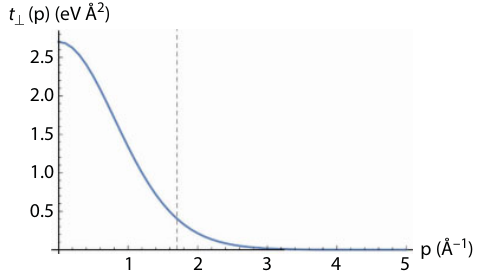
\includegraphics[width=0.6\linewidth]{fig/tperp.png}
\caption{Fourier transform for the interlayer hopping in tBLG. The vertical dashed line marks the position
of the Dirac point. Taken from \cite{handbook2019}.}
\label{fig:tperp}
\end{figure}

%%%%%%%%%%%%%%%%%%%%%%%%%%%%%%%%%%%%%%%%%%%%%%%%%%%%%%%%%%%%%%%%%%%%%%%%%%%%%%%%%%%%%%%%%%%%%%%%%%
\subsection{\textcolor{red}{Small rotation limit}}
%%%%%%%%%%%%%%%%%%%%%%%%%%%%%%%%%%%%%%%%%%%%%%%%%%%%%%%%%%%%%%%%%%%%%%%%%%%%%%%%%%%%%%%%%%%%%%%%%%

When the rotation angle $\theta \lesssim 10^\circ$ is small enough, we can expand around the Dirac points of each layer $\k_\ell = \K_\ell + \q_\ell$ with $\abs{\q_\ell} \sim \abs{\Delta \K} \ll \abs{\K}$. Approximating $t_\perp(\K_1+\q_1+\G_1) \approx t_\perp(\K_1+\G_1)$, the interlayer coupling becomes
$$
T_{12}^{\alpha\beta}(\q_1,\q_2) = \frac{1}{A_{\text{u.c.}}} \sum_{\G_1,\G_2} e^{i\G_1\vdot\vtau_{1,\alpha}}
t_{12}^{\alpha\beta}(\K_1+\G_1) e^{-i\G_2\vdot\vtau_{2,\beta}}
\delta_{\K_1+\q_1+\G_1,\K_2+\q_2+\G_2}.
$$

As $t_\perp(\p)$ decays rapidly with $\abs{\p}$, we truncate $t_\perp(\p) \approx 0$ for $\abs{\p} > \abs{\K}$. This leaves us only three options for $\G_1$, being $\g_{11} = \0$, $\g_{12} = \b_{12}$, $\g_{13} = -\b_{11}$. These three vectors correspond to the three $\K$ equivalent points on the monolayer BZ. Because of the indifference between layer 1 and 2, the same goes for $\G_2$. Notice that $\abs{\K_1+\g_{1n}} = \abs{\K}$, because they are equivalent $\K$ points. Thus, the only quantity that matters is $t_\perp(\abs{\K})$. We have the term
$$
\delta_{\K_1+\q_1+\G_1,\K_2+\q_2+\G_2} = \delta_{\q_2-\q_1,\K_1-\K_2+\G_1-\G_2}.
$$
We call $\Delta\K = \K_1-\K_2$. Due to $\abs{\q_\ell} \ll \abs{\K}$, we only have that $\q_2-\q_1 = \K_1-\K_2+\G_1-\G_2$ if $\G_1 = \g_{1n}$ and $\G_2 = \g_{2n}$ have the same index $n$. Therefore, we have three possibilities
$$
\q_\text{b} = \K_1 - \K_2 = \abs{\Delta \K} \qty(0, -1),
$$
$$
\q_\text{tr} = (\K_1 - \K_2) + (\g_{12} - \g_{22}) = \abs{\Delta \K} \qty(\frac{\sqrt{3}}{2}, \frac{1}{2}),
$$

$$
\q_\text{tl} = (\K_1 - \K_2) + (\g_{13} - \g_{23}) = \abs{\Delta \K} \qty(-\frac{\sqrt{3}}{2}, \frac{1}{2}),
$$
where $\abs{\Delta \K} = 2 \sin(\theta/2) \abs{\K}$.

The interlayer coupling has only three terms
$$
T_{12}^{\alpha\beta}(\q_1,\q_2) =
T^{\alpha\beta}_{\q_\text{b}} \delta_{\q_1-\q_2, \q_\text{b}} +
T^{\alpha\beta}_{\q_\text{tr}} \delta_{\q_1-\q_2, -\q_\text{tr}} +
T^{\alpha\beta}_{\q_\text{tl}} \delta_{\q_1-\q_2, -\q_\text{tl}},
$$
where $T^{\alpha\beta}_{\q_n} = \frac{t_\perp(\abs{\K})}{A_{\text{u.c.}}} e^{i \g_{1n} \vdot \bm{\tau}_{1\alpha}}
e^{-i \g_{2n} \vdot \bm{\tau}_{2\beta}}$. Writing it in the $A, B$ basis we get
$$
T_{\q_\text{b}} = \frac{t_\perp(\abs{\K})}{A_{\text{u.c.}}}
\begin{pmatrix}
1 & 1 \\
1 & 1
\end{pmatrix},
$$
$$
\textcolor{red}{
T_{\q_\text{tr}} = \frac{t_\perp(\abs{\K})}{A_{\text{u.c.}}} e^{-i \g_{12} \vdot \vtau_0}
\begin{pmatrix}
e^{i\phi} & 1 \\
e^{-i\phi} & e^{i\phi}
\end{pmatrix},
}
$$
$$
\textcolor{red}{
T_{\q_\text{tl}} = \frac{t_\perp(\abs{\K})}{A_{\text{u.c.}}} e^{-i \g_{13} \vdot \vtau_0}
\begin{pmatrix}
e^{-i\phi} & 1 \\
e^{i\phi} & e^{-i\phi}
\end{pmatrix},
}
$$
with $\phi = 2\pi/3$.

%%%%%%%%%%%%%%%%%%%%%%%%%%%%%%%%%%%%%%%%%%%%%%%%%%%%%%%%%%%%%%%%%%%%%%%%%%%%%%%%%%%%%%%%%%%%%%%%%%
%%%%%%%%%%%%%%%%%%%%%%%%%%%%%%%%%%%%%%%%%%%%%%%%%%%%%%%%%%%%%%%%%%%%%%%%%%%%%%%%%%%%%%%%%%%%%%%%%%


%%%%%%%%%%%%%%%%%%%%%%%%%%%%%%%%% COMMENT THIS TO COMPILE main.tex %%%%%%%%%%%%%%%%%%%%%%%%%%%%%%%%
%%%-----
%%% Referências bibliográficas
%%%-----
%\addcontentsline{toc}{chapter}{\bibname}
%%\bibliographystyle{abntex2-num}
%\bibliography{citations}
%\bibliographystyle{ieeetr}
%\end{document}
%%%%%%%%%%%%%%%%%%%%%%%%%%%%%%%%% COMMENT THIS TO COMPILE main.tex %%%%%%%%%%%%%%%%%%%%%%%%%%%%%%%%
